\documentclass{article}

\usepackage{amsmath}
\usepackage[margin=1.25in]{geometry}
\usepackage{graphicx}
\usepackage{physics}

\title{Hopf Bifurcation Analysis of Coupled Oscillators}
\author{Thomas Malthouse}
\date{\today}
\renewcommand{\vec}{\mathbf}
\newcommand{\self}{{\text{sf}}}
\newcommand{\cpl}{\text{c}}



\begin{document}
    \maketitle

    \tableofcontents

    \section{The Problem}

    Given an optoelectronic loop as shown in figure \ref{oeloop}, described by parameters $\tau_{\self}$ (the self-feedback delay), $\tau_\text{c}$ (the coupling delay), $\gamma_{\self}$ (the self-feedback strength), $\gamma_\text{c}$ (the coupling strength), as well as the behavior of the band-pass filter $F$ and nonlinear modulator, we want to predict whether the system will exhibit oscillation, or damp any oscillation over time.

    This is obviously a very difficult problem to solve, with four free parameters and tight coupling between the loops. To simplify the problem, we will begin by setting $\gamma_{\text{c}}=0$, so that the loops are uncoupled and can evolve independently.

    \begin{figure}[t]
        \centering
        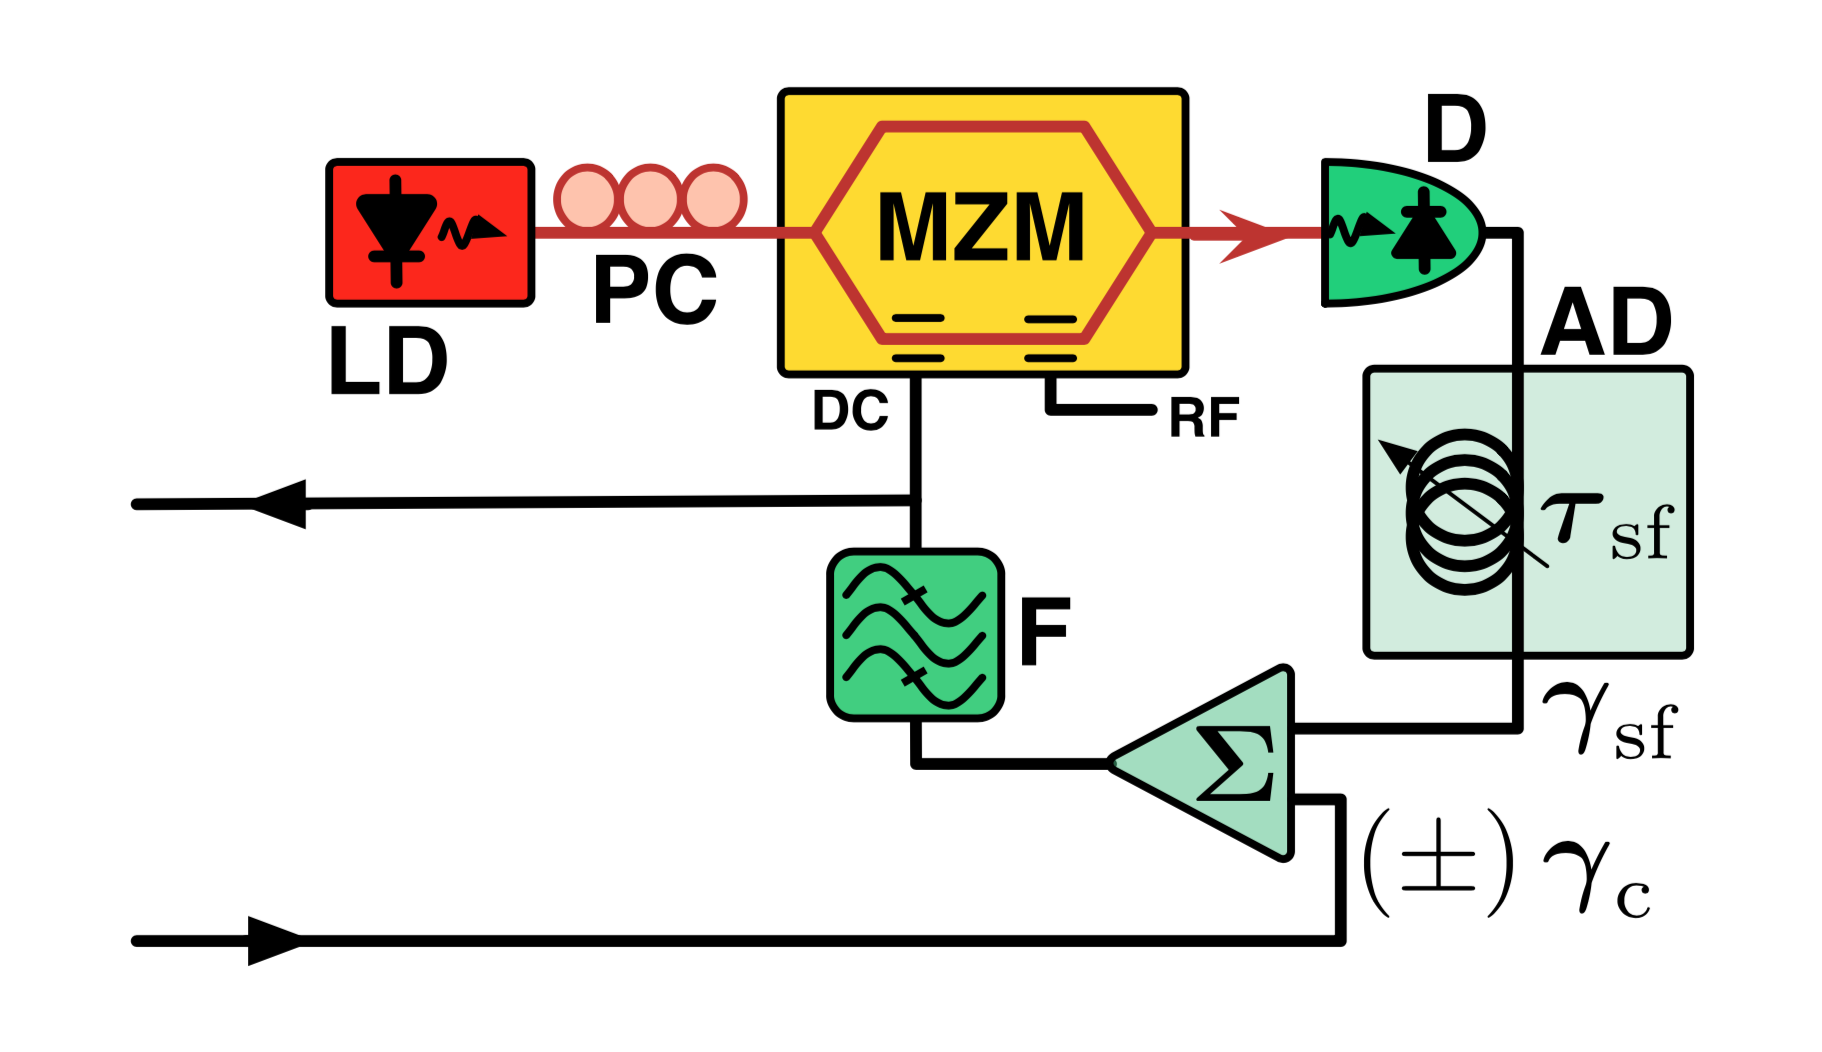
\includegraphics[width=0.5\textwidth]{figs/oeloop.png}
        \caption{The optoelectronic loop whose behavior we are hoping to characterize}
        \label{oeloop}
    \end{figure}

    \section{Uncoupled Oscillator Analysis}\label{uncoupledanalysis}

    Since the loops are identical, solving for the behavior of one is sufficient in the uncoupled case, since the second will behave identically. We can write down a pair of coupled differential equations that describe the uncoupled loop:

    \begin{equation}
        \begin{aligned}
            \dot{x} &= -x + y - \gamma_{11}f(x^{\tau_{11}}) \\
            \dot{y} &= \epsilon x
        \end{aligned}
    \end{equation}

    In this equation, $x$ is proportional to the signal strength, and $y$ proportional to the attenuation of the bandpass filter. $\epsilon$ described the bandpass filter, and is given by $\epsilon = \omega_0^2$, where $\omega_0$ is the center of the passband. $\gamma_{11}$ is a dimensionless quantity representing the strength of the self-coupling (though not equal to $\gamma_{\self}$ as described above!). $f$ is a function representing the behavior of the nonlinearity (in our case, a $\cos^2$ type relationship), and $x^{\tau_{11}}$ is shorthand for $x(t-\tau_{11})$.

    Assume the solution to these differential equations is
    \begin{equation}
        \begin{pmatrix}
            x \\ y
        \end{pmatrix} = 
        \begin{pmatrix}
            x_0 \\ y_0
        \end{pmatrix}e^{\lambda t}
    \end{equation}
    Plugging this solution in and linearizing the equation gives that

    \begin{equation*}
        \begin{aligned}
            \lambda x_0 e^{\lambda t} &= -x_0 e^{\lambda t} + y_0 e^{\lambda t} - \gamma_{11}f'(0)x_0 (e^{\lambda t}e^{-\lambda \tau_{11}}) \\
            \lambda y_0 &= \epsilon x_0
        \end{aligned}
    \end{equation*}
    Factor out $e^{\lambda t}$ from the first equation, and multiply both sides by $\lambda$ to give
    \begin{align}
        \lambda^2 x_0 &= -\lambda x_0 + \lambda y_0 - \lambda \gamma_{11}f'(0)x_0 e^{-\lambda \tau_{11}} \label{xeq1}\\
        \lambda y_0 &= \epsilon x_0 \label{yeq1}
    \end{align}
    We can then substitute eq. \ref{yeq1} into eq. \ref{xeq1}, giving
    \begin{align}
        \nonumber \lambda^2 x_0 &= -\lambda x_0 + \epsilon x_0 - \lambda \gamma_{11}f'(0)x_0 e^{-\lambda \tau_{11}} \\
        \nonumber \implies \lambda^2 &= -\lambda + \epsilon - \lambda \underbrace{\gamma_{11}f'(0)}_{=\gamma_\self}e^{-\lambda \tau_{11}} \\
        \label{leqrr} \implies 0 &= \lambda^2 + \lambda - \epsilon + \lambda \gamma_{\self}e^{-\lambda \tau_{11}}
    \end{align}
    Note that we now have the (physically measurable) $\gamma_\self$ parameter.

    Recall that we are interested in finding the critical curves along which the system transitions from damping to growing behavior. If $\Re(\lambda) > 0$, we will see divergent behavior, while $\Re(\lambda) < 0$ gives damping behavior---therefore, at points along the critical curve, $\Re(\lambda) = 0$. We can enforce this by saying $\lambda = i \Omega$, for real $\Omega$.

    Plugging this definition into eq. \ref{leqrr}, and separating the real and imaginary components yields two equations:
    \begin{align*}
        -\Omega^2 - \epsilon + \gamma_{\self}\Omega\sin(\Omega \tau_{11}) &= 0 \\
        \Omega + \gamma_\self\Omega \cos(\Omega \tau_{11}) &= 0
    \end{align*}
    Manipulating the second equation gives
    \begin{align*}
        0 &= 1 + \gamma_\self\cos(\Omega \tau_{11}) \\
        \gamma_\self &= -\frac{1}{\cos(\Omega \tau_{11})}
    \end{align*}
    so
    \begin{equation*}
        0 = \Omega^2 + \epsilon + \Omega\frac{\sin(\Omega \tau_{11})}{\cos(\Omega \tau_{11})} 
        = \Omega^2 + \epsilon + \Omega\tan(\Omega\tau_{11})
    \end{equation*}
    For a given $\tau$, then, we can solve for all valid values of $\Omega$, and use those to find the associated $\gamma$. (Typically, we draw the bifurcation plot with $\tau$ on the horizontal axis and $\gamma$ on the vertical, but this is just convention.)
    
    But wait! Note that each $\tau$ has an infinite number of $\gamma$s for which there is a valid solution (and v.v.), due to the periodicity of the trigonometric functions---giving us an infinite number of critical curves, as shown in figure \ref{omegas}. How do we determine which curve is the physical critical curve, where our actual, physical oscillator transitions from damping to growth?

    \begin{figure}[ht]
        \centering
        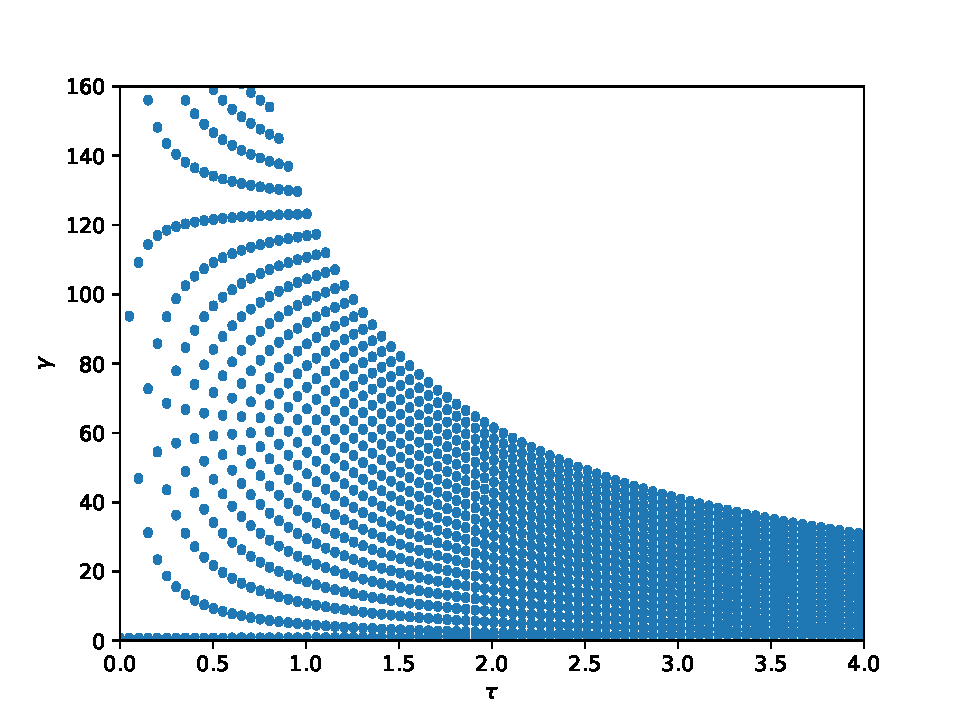
\includegraphics[width=0.7\textwidth]{figs/omegas.pdf}
        \caption{A subset of the (infinite) valid critical curves.}
        \label{omegas}
    \end{figure}

    Well, we know that $(\tau, \gamma) = (0,0)$ must exhibit damping, since (without any feedback) there can be no oscillation. We also don't care about solutions with negative $\tau$, since we can't look into the future. Therefore, the damping region consists of every point that can be reached from the origin without crossing a critical curve, and the physical critical curve consists of the smallest positive curve at each $\gamma$. 

    If we do this, we get something resembling figure \ref{physcrit}. Of course, that begs the question of how we \emph{know} that we have the lowest critical curve at each point---after all, with infinite curves, we need some heuristic to figure out whether we have the right curve. However, that's a question about numerical analysis, covered in a later section.

    \begin{figure}[ht]
        \centering
        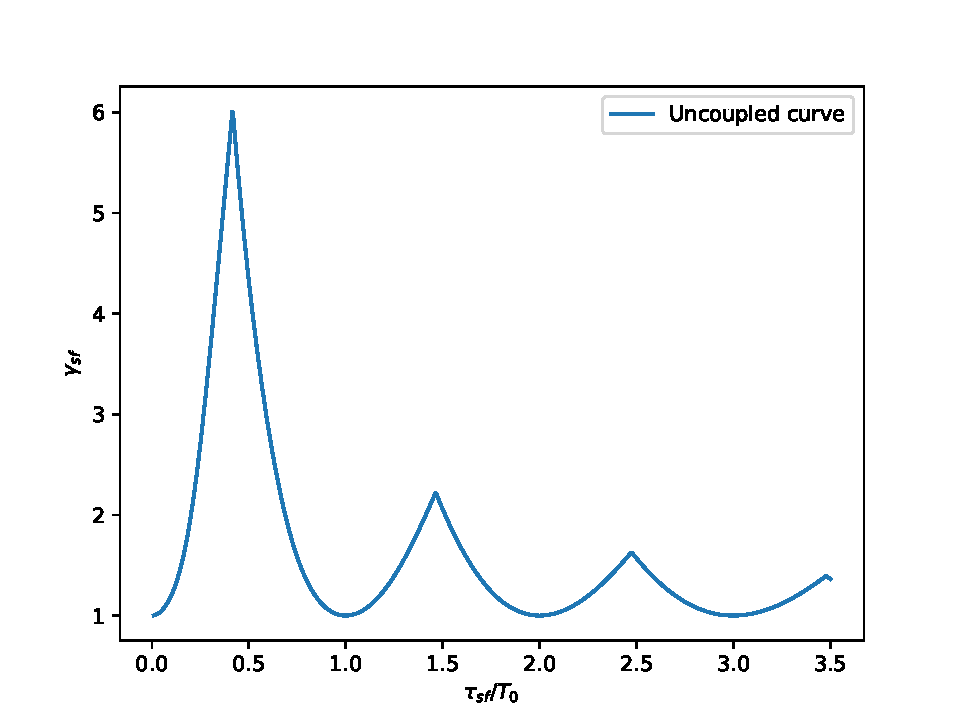
\includegraphics[width=0.7\textwidth]{figs/physical_critical.pdf}
        \caption{The physical curve, composed of the lowest critical curve at each point, stitched together}
        \label{physcrit}
    \end{figure}

    \section{Coupled Oscillator Analysis}

    The differential equations for the coupled case look very similar to those analyzed above---only now, there are four of them (two per oscillator), and there is an additional coupling term involved. With $u$ taking the place of $x$ above, and $v$ taking the place of $y$ (to avoid confusion), these equations can be written
    \begin{align*}
        \dot{u}_1 &= -u_1 + v_1 - \gamma_{11}f(u_{1}^{\tau_{11}}) + \gamma_{12}f(u_{2}^{\tau_{12}}) \\
        \dot{v}_1 &= \epsilon u_1 \\
        \dot{u}_2 &= -u_2 + v_2 - \gamma_{22}f(u_{1}^{\tau_{11}}) - \gamma_{21}f(u_{1}^{\tau_{21}}) \\
        \dot{v}_2 &= \epsilon u_2
    \end{align*}
    Note the opposite signs on the coupling terms.
    
    With this many variables floating around, writing the system as a matrix simplifies things. Let
    \begin{equation*}
        \vec{x} = \begin{pmatrix}
            u_1\\v_1\\u_2\\v_2
        \end{pmatrix}
    \end{equation*}
    and again assume $\vec{x} = \vec{x_0}e^{\lambda t}$. Performing the same linear approximation as above, we get that the system can be written as
    \begin{equation}
        \lambda \vec{x}_0 = \begin{pmatrix}
            -1-\gamma_{\self} e^{-\lambda \tau_{\self}} & 1 & \gamma_\cpl  e^{-\lambda \tau_\cpl} & 0 \\
            \epsilon & 0 & 0 & 0 \\
            -\gamma_\cpl  e^{-\lambda \tau_\cpl} & 0 & -1-\gamma_\self  e^{-\lambda \tau_\self} & 1\\
            0 & 0 & \epsilon & 0
        \end{pmatrix}
        \vec{x}_0 \equiv
        \vec{A}\vec{x}_0
    \end{equation}
    where $\gamma_{\self} = \gamma_{11}f'(0) = \gamma_{22}f'(0)$ and $\gamma_\cpl = \gamma_{12}f'(0) = \gamma_{21}f'(0)$.

    This is a transcendental eigenvalue problem, so let's try to solve it:
    \begin{align*}
        0 &=\det(\vec{A} - \lambda \vec{I}) \\
        %
        &= \left(
                1+\lambda + \gamma_\self e^{-\lambda\tau_\self}
            \right) \left(
            \lambda \left[
                \lambda \left(
                    1 + \gamma_\self e^{-\lambda \tau_\self} + \lambda
                \right) - \epsilon
            \right]
        \right) 
        - \epsilon \left[
            \lambda \left(
                1 + \gamma_\self e^{-\lambda \tau_\self} + \lambda
            \right) - \epsilon
        \right] 
        + \gamma_\cpl^2\lambda^2 e^{-2\lambda \tau_\cpl}
    \end{align*}
    Typically, we would solve this characteristic equation for $\lambda$ at this point. However, this isn't a nice, solvable polynomial like normal---the exponentials mean that there are infinite possible solutions. Instead, we can make assumptions about the value of $\lambda$, and use that to make inferences about the relationship between the other parameters.

    Just as in the uncoupled case, we know that $\lambda$ is purely imaginary on the boundary between damping and oscillatory behavior---that is, we can set $\lambda = i\Omega$ as before. Plugging that in, expanding everything out, and separating out the real and imaginary components, we get that
    \begin{align*}
        \intertext{Re:}
        0 &= -2\Omega^2 - 2 \Omega^2 \gamma_\self \cos(\Omega \tau_\self) + 2\Omega \gamma_\self \sin(\Omega \tau_\self) + \Omega\gamma_\self^2 \sin(2\Omega \tau_\self) \\&+ 2\Omega\epsilon\gamma_\self\sin(\Omega\tau_\self)-2\Omega^2\epsilon + \epsilon^2 - \gamma_\cpl^2\Omega^2\cos(2\Omega\tau_\cpl) \\
        \intertext{Im:}
        0 &= 1 - 2\Omega \gamma_\self \sin(\Omega\tau_\self) + 2\gamma_\self\cos(\Omega \tau_\self)
        + \gamma_\self^2\cos(2\Omega\tau_\self) \\&- \Omega^2 + 2\epsilon + 2\epsilon\gamma_\self\cos(\Omega\tau_\self) + \gamma_\cpl^2\Omega\sin(2\Omega\tau_\cpl)
    \end{align*}

    If we combine these two equations to eliminate $\gamma_\self$ and normalize, we get that, for points on the critical curve,
    \begin{equation}\label{taucpleq}
        0 = \Omega^2\cos(\Omega \tau_\self) + \Omega \left[1-\gamma_\cpl\sin(\Omega\tau_\cpl)\right]\sin(\Omega\tau_\self) - \epsilon + \gamma_\cpl \Omega \cos(\Omega\tau_\cpl)\cos(\Omega\tau_\self)
    \end{equation}
    Then, for a particular value of $\Omega$, the associated $\gamma_\self$ is
    \begin{equation}\label{gammacpleq}
        \gamma_\self = \frac{1-\gamma_\cpl\sin(\Omega \tau_\cpl)}{\cos(\Omega \tau_\self)}
    \end{equation}

    \section{Numerical Analysis}
    We now have equations that can tell us, both in the uncoupled and coupled cases, whether a given $\Omega$ lies on the critical curve at some $\tau$, and the $\gamma$ associated with that $\Omega$. However, as described at the end of section \ref{uncoupledanalysis}, we only care about the \emph{lowest} critical point for each $\tau$---and there is no easy way to determine whether a given critial point is actually the lowest.

    \subsection{The Naive Problem}
    At first, this problem seems relatively simple. We know the combined critical curve (fig. \ref{physcrit}) must be continuous---otherwise, it would be nonphysical and lead to some strange behavior. Given a point $\gamma_n$ on the curve at $\tau_n$, we could carefully search the interval
    \begin{equation*}
        [\gamma_n -\varepsilon, \gamma + \varepsilon]
    \end{equation*}
    for a valid solution at $\tau_{n+1}$. If more than one valid solution is found in this interval, we (of course) prefer the smaller one---allowing us to detect the point where curves cross. With careful choice of $\tau$ spacing and $\varepsilon$, we should be able to follow the critical curve.

    Unfortunately, things are never that simple. Given a gamma, there is \emph{no way} to check whether it lies on a critical curve. As seen in equations \ref{taucpleq} and \ref{gammacpleq}, both $\tau$ and $\gamma$ are parameterized by $\Omega$, and neither of these equations has an inverse (at least in the coupled case). Determining whether $(\tau,\gamma)$ lies on a critical curve requires determining whether there is any $\Omega$ (which, again, could be any real number) that satisfies both equations \ref{taucpleq} and \ref{gammacpleq}. 

    \subsection{Bounding $\Omega$}



\end{document}